\section{HySparse2}

\subsection{Overview}

Figure~\ref{fig:hysparse2-overview} illustrates the HySparse2 architecture.
Following YOCO~\citep{yoco}, the backbone is divided into a self-decoder and a cross-decoder.
Both decoders use hybrid attention.
The self-decoder hybridizes full attention with sliding-window attention for local modeling.
The cross-decoder hybridizes full attention with sparse attention for global retrieval.
HySparse2 uses two-level KV sharing.
At the outer level, \textbf{KV Bridging} constructs each cross-decoder full-attention layer's KV cache from corresponding self-decoder hidden states through layer-specific projections.
At the inner level, \textbf{KV Reuse} lets sparse layers reuse the full-attention layer's KV cache and selection indices within each hybrid block.

\begin{figure}[!t]
    \centering
    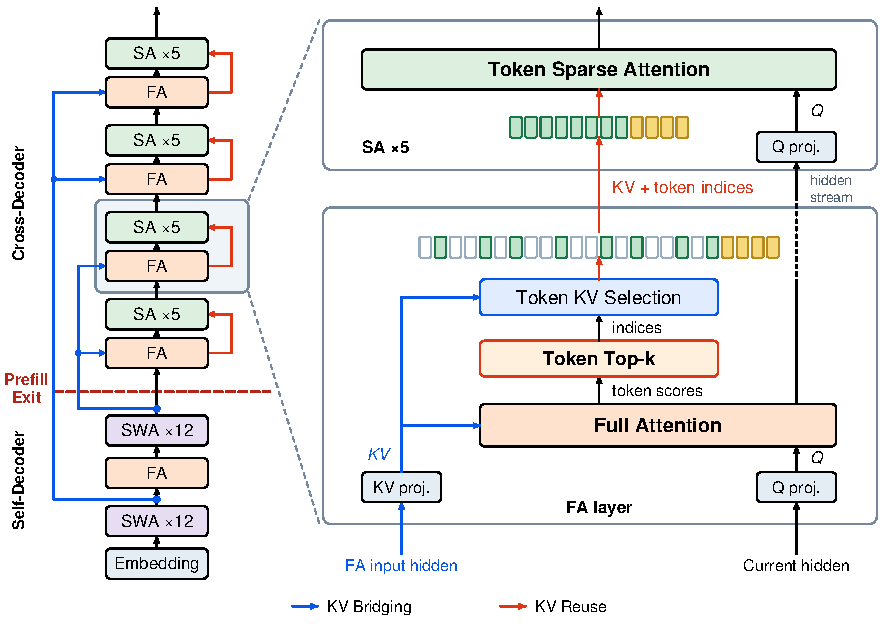
\includegraphics[width=\linewidth]{figures/hysparse2-architecture.pdf}
    \caption{Two-level KV sharing in HySparse2. FA, SWA, and SA denote full attention, sliding-window attention, and sparse attention, respectively. Left: the overall architecture with KV Bridging between the self-decoder and cross-decoder. Prefill cache construction can exit after the self-decoder. Right: a HySparse2 block with token-level sparse attention and a forced local window. Through KV Reuse, SA layers reuse the block’s FA KV cache and selection indices.}
    \label{fig:hysparse2-overview}
\end{figure}

\subsection{Full-Attention-Only KV Bridging}
\label{sec:kv-bridging}

KV Bridging operates only between full-attention layers in the self-decoder and cross-decoder.
Consider a pair of full-attention layers $(i,j)$, with layer $i$ in the self-decoder and layer $j$ in the cross-decoder.
Let $\mathbf{H}^{\mathrm{self}}_i$ and $\mathbf{H}^{\mathrm{cross}}_j$ denote the corresponding input hidden states.
Cross-decoder layer $j$ computes its keys, values, and queries as
\begin{equation}
    \mathbf{K}^{\mathrm{cross}}_j = \operatorname{Proj}^{K}_{j}\!\left(\mathbf{H}^{\mathrm{self}}_i\right), \quad
    \mathbf{V}^{\mathrm{cross}}_j = \operatorname{Proj}^{V}_{j}\!\left(\mathbf{H}^{\mathrm{self}}_i\right), \quad
    \mathbf{Q}^{\mathrm{cross}}_j = \operatorname{Proj}^{Q}_{j}\!\left(\mathbf{H}^{\mathrm{cross}}_j\right).
\end{equation}
Each cross-decoder full-attention layer has its own K/V projections, so layers that share a hidden-state source still construct distinct KV caches.
Each layer also retains an independent Q projection applied to its own current hidden states.
KV Bridging supports different hybrid attention ratios in the two decoders, allowing one self-decoder full-attention layer to supply multiple cross-decoder full-attention layers, as illustrated in Figure~\ref{fig:hysparse2-overview}.

\subsection{Cross-Layer KV Reuse}
\label{sec:kv-reuse}

HySparse2 makes two key refinements to HySparse: adopting token-level sparse selection and removing the separate SWA branch.

\paragraph{Token-Level Sparse Selection.}

In HySparse, pretraining evaluations showed no substantial accuracy disadvantage for block-level selection.
However, block-level sparsity shows a pronounced accuracy disadvantage on multi-turn, long-context agentic tasks.
HySparse2 therefore applies top-$k$ selection to individual tokens in full-attention layers, and the following sparse layers reuse the KV entries for the selected tokens.
Section~\ref{sec:token-block-ablation} evaluates selection granularity.

\paragraph{Removing the Separate SWA Branch.}

HySparse2 removes the separate SWA branch used in HySparse and supports local modeling by forcing a recent window into the sparse selection.
As illustrated in Figure~\ref{fig:hysparse2-overview}, a local window of the most recent tokens is always selected, followed by the highest-scoring tokens outside the window.
Both selected sets are read from the full-attention KV cache and reused by the following sparse-attention layers.

This design also enables a complete early exit after the self-decoder during prefill. A separate SWA branch in the cross-decoder requires building a suffix of KV cache from projections of its own hidden states, which further depends on an expanding set of hidden states in earlier layers and grows linearly with depth. This cascading SWA dependency therefore requires the cross-decoder to process a token suffix far longer than the window size. The required states must either be computed during prefill, preventing the cross-decoder from being skipped entirely, or approximated by methods such as bounded replay~\citep{deepseekv41flash}. HySparse2 removes this dependency by construction and requires no cross-decoder computation during prefill. Removing the branch also eliminates substantial parameter overhead from the separate projections in our gated baseline.

\subsection{The Role of Full Attention}
Both HySparse2 and HySparse retain a small number of full-attention layers, as we believe that full attention remains important for model quality. 
These full-attention layers also serve as indexers, using exact attention scores to provide oracle token selection for subsequent sparse layers.
This design supports native end-to-end training without a separate indexer or an auxiliary distillation objective to train one.
Full attention nevertheless remains computationally expensive, so we keep the proportion of full-attention layers small. In HySparse2, prefill KV-cache construction requires only one full-attention layer. Following recent sparsification approaches~\citetext{\citealp{seerattn_v1}; \citealp{dsa}}, we could further approximate the retained full-attention layers with a lightweight indexer plus sparse attention in post-training.
Future architectures could also allocate less computation to full attention and more to sparse attention, for example by reducing the number of query heads in full-attention layers while increasing it in sparse-attention layers.


\subsection{Inference Architecture}
\label{sec:prefill-decode}

\paragraph{Prefill–Decode Disaggregation.}

Under prefill--decode disaggregation, the HySparse2 prefill node hosts only the self-decoder and the KV Bridging projections.
For the 49-layer model shown in Figure~\ref{fig:hysparse2-overview}, this requires deploying only the first 25 layers, cutting the memory requirement of the prefill node by nearly half.
With a high SWA-to-full-attention ratio, the self-decoder performs full attention in only one layer during the prefill stage.
We also compute the cross-decoder full-attention KV caches on the prefill node and transfer them to the decode nodes, because the projected KV caches are smaller than the source hidden states.

\paragraph{Speculative Decoding.}

During pretraining, HySparse2 uses a single MTP layer conditioned on the hidden states at the self-decoder/cross-decoder boundary to aid convergence.
During post-training, this MTP layer could be replaced with a larger DFlash-style drafter conditioned on the same hidden states~\citep{chen2026dflash}.
Their early availability could support asynchronous drafting and verification~\citep{zhang2025swiftspec}.
Training the larger drafter and coordinating asynchronous execution with verification feedback remain future work.

